\section{Rauschen}


\subsection{Rauschen in der Elektronik}

\begin{outline}
    \1 \textbf{Alle Teile eines elektronischen Systems rauschen!}
    \1 Messpfad: Es sollen keine Störsignale zum Messsignal addiert werden
        \2 Ausser bei perfekter Abschirmung und Temperatur $0 \, \kelvin$ gibt es \textbf{immer} Störeinflüsse
    \1 \textbf{ADC} und DAC: Quantisierungsrauschen $q$ (Quantisierungsschritt)
        \2 Quantisierungsrauschen (Auflösung) soll etwa so gross gewählt werden, wie das elektronische Rauschen
    \1 'Reine DC-Spannungen' gibt es nicht!
        \2 Auch DC-Signale haben Spannungs-Schwankungen
\end{outline}


\subsection{Arten von Rauschen}

\begin{minipage}[t]{0.48\columnwidth}
    \begin{itemize}
        \item \textbf{Thermisches Rauschen}
        \item \textbf{Flicker Noise} $\frac{1}{f}$-Noise
    \end{itemize}
\end{minipage}
\hfill
\begin{minipage}[t]{0.48\columnwidth}
    \begin{itemize}
        \item Shot Noise
        \item Burst (Popcorn) Noise
        \item Avalanche Noise
    \end{itemize}
\end{minipage}


\subsubsection{Thermisches Rauschen}

\begin{outline}
    \1 Entsteht durch \textbf{zufällige Bewegung der Ladungsträger} aufgrund der \textbf{Wärmeenergie}
        und der \textbf{Quantisierung der Ladung}
    \1 Ist über die Frequenzen \textbf{gleichverteilt}
    \1 Begriff: Weisses Rauschen
        \2 Anderer Ausdruck: Johnson Noise
\end{outline}


\subsubsection{Flicker Noise (Funkelrauschen)}

\begin{outline}
    \1 Entsteht am \textbf{Übergang} von zwei Materialien
        \2 u.a. in MOS-FET, wenn isch Elekronen in Fehlerstellen zw. Silizium und Gate-Oxid oder zw. Gate-Oxid 
            und Gate verfangen und nach gewissen Zeit zufällig wieder freikommen
    \1 Rauschleistung nimmt \textbf{umgekehrt proportional zur Frequenz ab} \textrightarrow\ $\frac{1}{f}$-Noise
    \1 Jede Dekade liefert die gleiche Rauschleistung
\end{outline}


\subsection{Amplitude und Leistung des Rauschens}

\textbf{Hinweis:} Als 'Leistung' gilt die \textbf{quadrierte Spannung}

\renewcommand{\arraystretch}{2}
\begin{tabular}{ll}
    Mittelwert der Rauschspannung       & $\overline{v_n}(t) = \frac{1}{T} \int_T v_n(t) \, \diff t \bm{= 0}$ \\
    Mittelwert der Leistung (Varianz)   & $\overline{v_n(t)^2} = \frac{1}{T} \int_T v_n^2(t) \, \diff t \bm{\neq 0}$ \\
    Effektivwert (Wurzel der Varianz)   & $\overline{v_{n, \rm rms}} = \sqrt{\overline{v_n(t)^2}} $\\
\end{tabular}
\renewcommand{\arraystretch}{1}


\subsubsection{Berechnung von Rauschen (!)}

\begin{outline}
    \1 Signale und Rauschen addieren sich \textbf{nicht gleich}
        \2 Deterministische \textbf{Signale}: \textbf{Amplituden} addieren sich
        \2 Stochastische Rauschquellen: \textbf{Rauschleistungen} addieren sich
\end{outline}


\subsection{Rauschen von Widerständen}

\begin{itemize}
    \item \textbf{Jeder Widerstand rauscht, unabhängig vom Stromfluss}
    \item Rauschen kann auf folgende zwei Arten modelliert werden
\end{itemize}

\begin{minipage}[c]{0.15\columnwidth}
    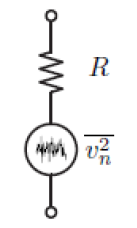
\includegraphics[width=\columnwidth]{images/rauschquelle_spannung.png}
\end{minipage}
\hfill
\begin{minipage}[c]{0.21\columnwidth}
    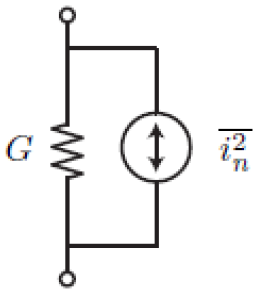
\includegraphics[width=\columnwidth]{images/rauschquelle_strom.png}
\end{minipage}
\hfill
\begin{minipage}[c]{0.62\columnwidth}
    \begin{minipage}[c]{0.48\columnwidth}
        $$ \boxed{ \overline{v_n^2} = 4 k T R B } $$
    \end{minipage}
    \hfill
    \begin{minipage}[c]{0.48\columnwidth}
        $$ \boxed{ \overline{i_n^2} = 4 k T G B } $$
    \end{minipage}
    \vspace{0.2cm}

    \begin{tabular}{l l c}
        $\overline{v_n^2}$  & mittlere Rauschleistung   & $[\overline{v_n^2}] = \volt^2$ \\
        $\overline{i_n^2}$  & mittlerer Rauschleistung  & $[\overline{i_n^2}] = \ampere^2$ \\ % CHECK heisst das so? Eineheit?
        $R$                 & Widerstand                & $[R] = \ohm$ \\
        $G$                 & Leitwert                  & $[G] = \siemens$ \\
        $B$                 & Bandbreite                & $[B] = \hertz$ \\
        $T$                 & absolute Temperatur       & $[T] = \kelvin$ \\
        \end{tabular}
        \begin{tabular}{ll}
        $k$                 & Boltzmann-Konstante $k = 1.38 \cdot 10^{-23} \, \frac{\joule}{\kelvin}$ \\
    \end{tabular}
\end{minipage}


\subsubsection{Serieschaltung von Widerständen}

\begin{minipage}[c]{0.4\columnwidth}
    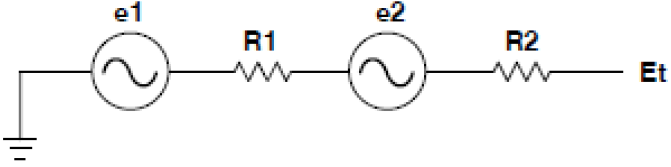
\includegraphics[width=\columnwidth]{images/serieschaltung_rauschende_widerstaende.png}
\end{minipage}
\hfill
\begin{minipage}[c]{0.58\columnwidth}
    \begin{minipage}[c]{0.48\columnwidth}
        $$ \boxed{ \overline{E_t^2} = \overline{e_1^2} + \overline{e_2^2} } $$
    \end{minipage}
    \hfill
    \begin{minipage}[c]{0.48\columnwidth}
        $$ [E_t] = \volt^2 $$
    \end{minipage}
\end{minipage}

\textbf{Nicht die Rauschspannungen, sondern die Rauschleistungen $\bm{e_i}$ müssen addiert werden!}


\subsection{Rauschen von Spannungsteilern}

\begin{minipage}[c]{0.13\columnwidth}
    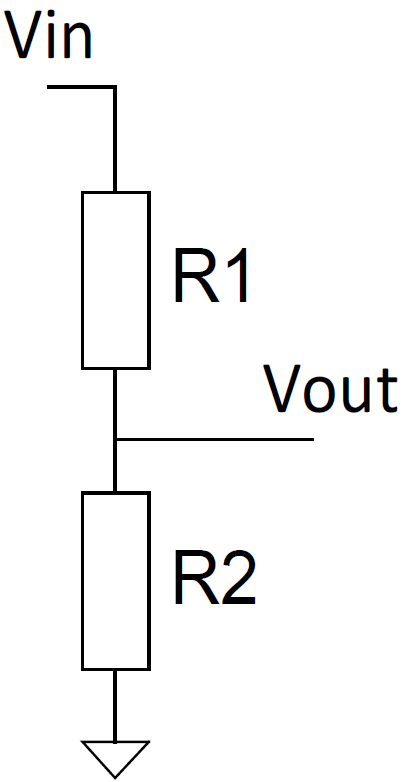
\includegraphics[width=\columnwidth]{images/rauschen_spannungsteiler.png}
\end{minipage}
\hfill
\begin{minipage}[c]{0.8\columnwidth}
    Rauschquellen sind \textbf{Kleinsignalquellen!} \textrightarrow\ $V_{\rm in} =$ GND
    $$ \boxed{\text{Rauschleistung:} \quad E_{\rm Vout} = 4 k T \cdot \frac{R_1 \cdot R_2}{R_1 + R_1} } $$
    $$ \boxed{\text{Rauschspannung:} \quad V_{\rm rausch} = \sqrt{E_{\rm Vout} } } $$
\end{minipage}


\subsection{Vorgehen Gesamt-Rauschen berechnen}

\begin{itemize}
    \item Lastwiderstände der Schaltung 'abhängen'
    \item Spannungs- und Stromquellen 'ausschalten'
    \item Von $R_L$ 'in Schaltung hineinschauen und Ersatzwiderstand $R_T$ berechnen
    \item Rauschleistung und ev. Rauschspannung berechnen
\end{itemize}


\subsubsection{Tipps und Tricks}    %CHECK ob das so stimmt

\begin{outline}
    \1 \textbf{Impedanzen}(Kondensatoren, Spulen)
        \2 Rausch\textbf{leistung} berechnen (per Integral, da Impendanz variabel in Frequenz)
    \1 \textbf{Parallelschaltung} von Widerständen / Impedanzen
        \2 Rauschleistungen der einzelnen Komponenten separat berechnen
        \2 Einzelne Rauschleistungen \textbf{addieren}
        \2 Falls Rauschspannung gesucht: Wunzel ziehen 
\end{outline}


\example{Gesamt-Rauschen berechnen}

\begin{minipage}[c]{0.28\columnwidth}
    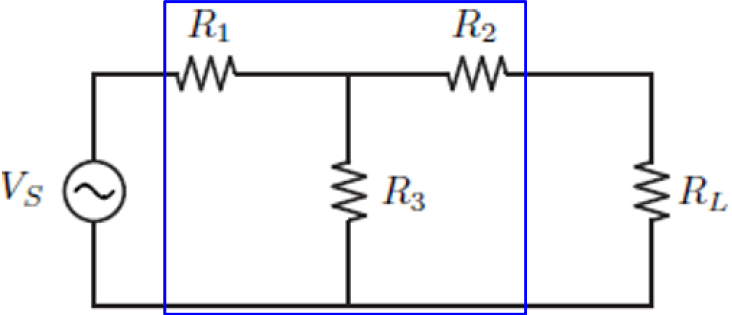
\includegraphics[width=\columnwidth]{images/gesamte_rauschspannung_schaltung.png}
\end{minipage}
\hfill
\begin{minipage}[c]{0.22\columnwidth}
    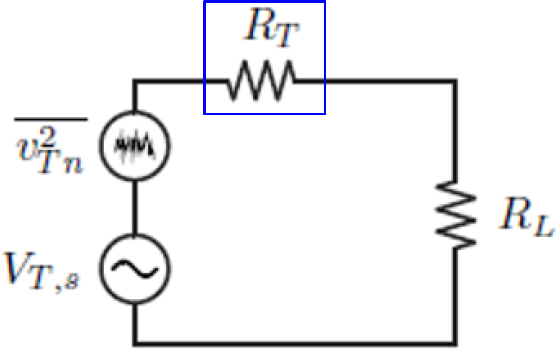
\includegraphics[width=\columnwidth]{images/gesamte_rauschspannung_ersatzschaltung.png}
\end{minipage}
\hfill
\begin{minipage}[c]{0.48\columnwidth}
    \renewcommand{\arraystretch}{1.4}
    \begin{tabular}{ll@{}}
        Ersatzwiderstand:   & $R_T = R_2 + R_1 || R_3$      \\
        Rauschleistung:     & $v^2_{Tn} = 4 k R_T B $       \\
        Rauschspannung:     & $v_{Tn} = \sqrt{v^2_{Tn}}$    \\
    \end{tabular}
    \renewcommand{\arraystretch}{1}
\end{minipage}


% \subsection{Rauschspannung und Rauschleistungsdichte} 
% TODO: Fragen wegen Slide 21 und dann ev. ergänzen


\subsection{Rauschbandbreite}
% TODO: formatting -> blöder Seitenumbruch in Gesamtdokumet
\begin{itemize}
    \item In Realität werden Signal und Rauschen Tiefpass-gefiltert
    \item \textbf{Rauschbandbreite nicht identisch mit $\bm{3 \, \deci \bel}$-Bandbreite!} \\
        \textrightarrow\ ENB (Effective Noise Bandwidth)
\end{itemize}

\vspace{0.2cm}
Für $n$ kaskadierte Butterworth-Filter 1. Ordnung mir Grenzfrequenz $f_c = \frac{1}{2 \pi R C}$ verhält sich das ENB gemäss:

\begin{minipage}[c]{0.6\columnwidth}
    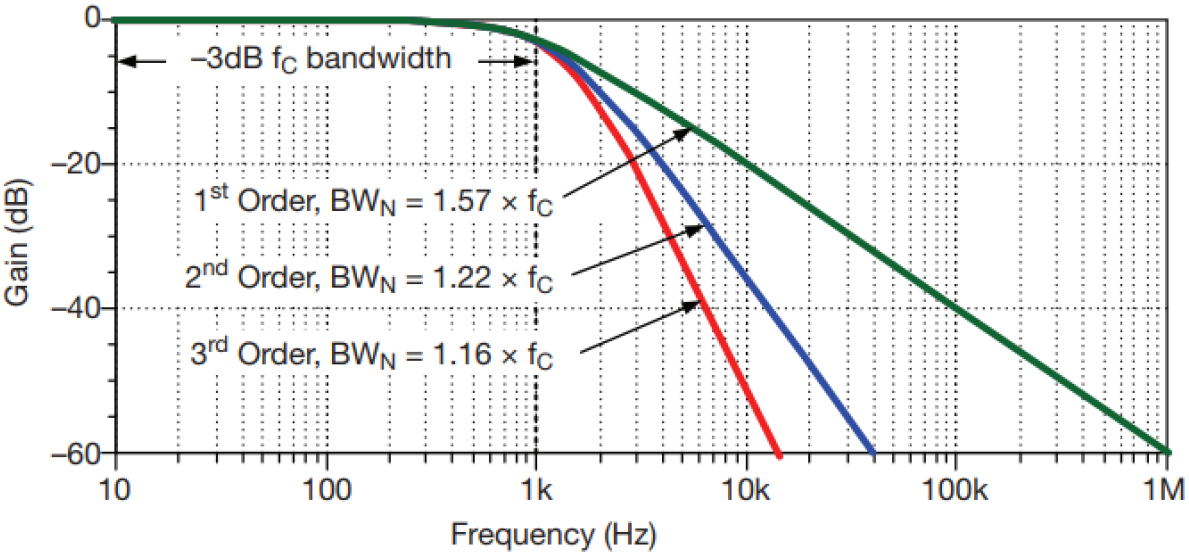
\includegraphics[width=\columnwidth]{images/rausch_bandbreite.png}
\end{minipage}
\hfill
\begin{minipage}[c]{0.38\columnwidth}
    \begin{tabular}{c | c}
        \toprule
        \textbf{Filterordnung}  & \textbf{ENB} \\
        \midrule
        $1$                     & $1.57 \cdot f_c$ \\
        \midrule
        $2$                     & $1.11 \cdot f_c$ \\
        \midrule
        $3$                     & $1.05 \cdot f_c$ \\
        \midrule
        $4$                     & $1.025 \cdot f_c$ \\
        \bottomrule
    \end{tabular}

\end{minipage}